\documentclass[
11pt, % The default document font size, options: 10pt, 11pt, 12pt
codirector, % Uncomment to add a codirector to the title page
]{charter} 




% El títulos de la memoria, se usa en la carátula y se puede usar el cualquier lugar del documento con el comando \ttitle
\titulo{Sistema de control para un robot tetrápodo} 

% Nombre del posgrado, se usa en la carátula y se puede usar el cualquier lugar del documento con el comando \degreename
%\posgrado{Carrera de Especialización en Sistemas Embebidos} 
%\posgrado{Carrera de Especialización en Internet de las Cosas} 
%\posgrado{Carrera de Especialización en Intelegencia Artificial}
\posgrado{Maestría en Sistemas Embebidos} 
%\posgrado{Maestría en Internet de las cosas}

% Tu nombre, se puede usar el cualquier lugar del documento con el comando \authorname
\autor{Ing. Pablo Daniel Folino} 

% El nombre del director y co-director, se puede usar el cualquier lugar del documento con el comando \supname y \cosupname y \pertesupname y \pertecosupname
\director{Ing. Juan Carlos Gómez}
\pertenenciaDirector{INTI,UTN.BA} 
% FIXME:NO IMPLEMENTADO EL CODIRECTOR ni su pertenencia
\codirector{} % para que aparezca en la portada se debe descomentar la opción codirector en el documentclass
\pertenenciaCoDirector{}

% Nombre del cliente, quien va a aprobar los resultados del proyecto, se puede usar con el comando \clientename y \empclientename
\cliente{Ing. Claudio Verrastro}
\empresaCliente{UTN-FRBA-GIAR}

% Nombre y pertenencia de los jurados, se pueden usar el cualquier lugar del documento con el comando \jurunoname, \jurdosname y \jurtresname y \perteunoname, \pertedosname y \pertetresname.
\juradoUno{Nombre y Apellido (1)}
\pertenenciaJurUno{pertenencia (1)} 
\juradoDos{Nombre y Apellido (2)}
\pertenenciaJurDos{pertenencia (2)}
\juradoTres{Nombre y Apellido (3)}
\pertenenciaJurTres{pertenencia (3)}
 
\fechaINICIO{21 de junio de 2021}		%Fecha de inicio de la cursada de GdP \fechaInicioName
\fechaFINALPlan{20 de agosto de 2021} 	%Fecha de final de cursada de GdP
\fechaFINALTrabajo{22 de agosto de 2022}	%Fecha de defensa pública del trabajo final


\begin{document}

\maketitle
\thispagestyle{empty}
\pagebreak


\thispagestyle{empty}
{\setlength{\parskip}{0pt}
\tableofcontents{}
}
\pagebreak


\section*{Registros de cambios}
\label{sec:registro}


\begin{table}[ht]
\label{tab:registro}
\centering
\begin{tabularx}{\linewidth}{@{}|c|X|c|@{}}
\hline
\rowcolor[HTML]{C0C0C0} 
Revisión & \multicolumn{1}{c|}{\cellcolor[HTML]{C0C0C0}Detalles de los cambios realizados} & Fecha      \\ \hline
0      & Creación del documento                                 &\fechaInicioName \\ \hline
1      & Se completa hasta el punto 2 inclusive                 & 25 de junio de 2021 \\ \hline
2      & Se completa hasta el punto 7 inclusive					& 02 de julio de 2021 \\ \hline
3	   & Se completa hasta el punto 10 inclusive 				& 06 de julio de 2021 \\ \hline
4	   & Se corrige hasta el punto 10 inclusive 				& 29 de julio de 2021 \\ \hline
5	   & Se completa hasta el punto 11 inclusive 				& 02 de agosto de 2021 \\ \hline
6	   & Se completa hasta el punto 15 inclusive 				& 04 de agosto de 2021 \\ \hline
%		  En distintas líneas \newline
%		  Así                                                    & dd/mm/aaaa \\ \hline
%3      & Se completa hasta el punto 11 inclusive                & dd/mm/aaaa \\ \hline
%4      & Se completa el plan	                                 & dd/mm/aaaa \\ \hline
\end{tabularx}
\end{table}

\pagebreak

\section*{Acta de constitución del proyecto}
\label{sec:acta}

\begin{flushright}
Buenos Aires, \fechaInicioName
\end{flushright}

\vspace{2cm}

Por medio de la presente se acuerda con el Ing. \authorname\hspace{1px} que su Trabajo Final de la \degreename\hspace{1px} se titulará ``\ttitle'', consistirá esencialmente en la implementación de un prototipo de un sistema de control de movimientos para un robot tetrápodo de tres grados de libertad en cada extremo, y tendrá un presupuesto preliminar estimado de 600 hs de trabajo y \$285.472, con fecha de inicio \fechaInicioName\hspace{1px} y fecha de presentación pública \fechaFinalName.

Se adjunta a esta acta la planificación inicial.

\vfill

% Esta parte se construye sola con la información que hayan cargado en el preámbulo del documento y no debe modificarla
\begin{table}[ht]
\centering
\begin{tabular}{ccc}
\begin{tabular}[c]{@{}c@{}}Ariel Lutenberg \\ Director posgrado FIUBA\end{tabular} & \hspace{2cm} & \begin{tabular}[c]{@{}c@{}}\clientename \\ \empclientename \end{tabular} \vspace{2.5cm} \\ 
\multicolumn{3}{c}{\begin{tabular}[c]{@{}c@{}} \supname \\ Director del Trabajo Final\end{tabular}} \vspace{2.5cm} \\
%\begin{tabular}[c]{@{}c@{}}\jurunoname \\ Jurado del Trabajo Final\end{tabular}     &  & \begin{tabular}[c]{@{}c@{}}\jurdosname\\ Jurado del Trabajo Final\end{tabular}  \vspace{2.5cm}  \\
%\multicolumn{3}{c}{\begin{tabular}[c]{@{}c@{}} \jurtresname\\ Jurado del Trabajo Final\end{tabular}} \vspace{.5cm}                                                                     
\end{tabular}
\end{table}




\section{1. Descripción técnica-conceptual del proyecto a realizar}
\label{sec:descripcion}


%\begin{consigna}{red} % El bloque "consigna" se usa para poner texto en rojo y dar una pequeña ayuda sobre cómo completar la sección

%El objetivo es que el lector en una o dos páginas entienda de qué se trata el proyecto y cuáles son sus desafíos, su motivación y su importancia.

%Se debe destacar claramente cuál es el valor que agrega el proyecto a realizar. ``El presente proyecto se destaca especialmente por incorporar tal cosa... Esto lo diferencia de otros sistemas similares en que ...''

%Puede ser útil incluir en esta sección la respuesta a alguna de estas preguntas:

%\begin{itemize}
%	\item ¿Cómo se vincula este proyecto con la misión de la organización?
%	\item ¿Cómo se inserta este proyecto en el modelo de negocio de la organización?
%	\item ¿Ayuda a la explicación si se incluye un lienzo Canvas del Modelo de Negocio?
%	\item ¿En qué estado del ciclo de vida está el producto que se desea reemplazar o mejorar?
%	\item ¿Cuáles son las necesidades que debe satisfacer?
%	\item ¿Por dónde pasa la innovación?
%\end{itemize}

%La descripción técnica-conceptual \textbf{debe incluir al menos un diagrama en bloques %del sistema} y una frase como la siguiente: ``En la Figura \ref{fig:diagBloques} se %presenta el diagrama en bloques del sistema. Se observa que...''. Luego recién más %abajo de haber puesto esta frase, se pone la figura. La regla es que las figuras nunca %pueden ir antes de ser mencionadas en el texto, porque sino el lector no entiende por %qué de pronto aparece una figura.

%\vspace{25px}



%\begin{figure}[htpb]
%\centering 
%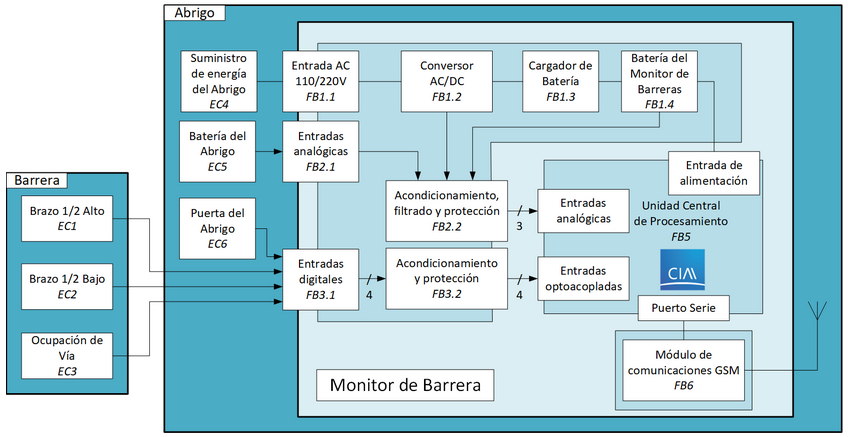
\includegraphics[width=.5\textwidth]{./Figuras/diagBloques.png}
%\caption{Diagrama en bloques del sistema}
%\label{fig:diagBloques}
%\end{figure}

%\vspace{25px}

%El tamaño de la tipografía en TODAS las figuras debe ser adecuado para que NO pase lo que ocurre acá, %donde el lector debe esforzarse para poder leer el texto. Los colores usados en el diagrama deben ser %adecuados, tal que ayuden a comprender mejor el diagrama, preferentemente en la gama de colores pastel.
%\end{consigna}


El objetivo es diseñar el hardware y firmware para controlar los movimientos de un robot tetrápodo de tres grados de libertad por cada extremo. El cerebro del sistema será una placa de desarrollo a definir, que recibirá la información de los distintos sensores y controlará los actuadores. La placa recibirá información de comunicación por un módulo Wi-Fi (del tipo ESP8266).
Esta placa de desarrollo, tendrá la suficiente potencia de procesamiento como para manejar la comunicación, todos los sensores y actuadores para el normal funcionamiento del robot. 

En las articulaciones se utilizarán servomtores controlados por modulación de ancho de pulso(PWM-\textit{Pulse-width modulation}). 

El sistema (hardware-software) tiene que ser robusto para que permita realizar las distintas pruebas a las que se va a someter.

Uno de los principales problemas de los robots caminantes es su estabilidad, para ello se utilizara un módulo acelerómetro. Otro de los problemas es el consumo de los servomotores, por lo qué el sistema medirá la corriente de cada articulación.   

La generación y control de la locomoción en robots caminantes requiere de un esfuerzo computacional alto, tanto en el diseño como en la implementación. Es necesario coordinar los movimientos y trayectorias de todas las articulaciones de las extremidades del robot; lo cual resulta especialmente complicado cuando el número de extremidades aumenta, para ello se aplicarán algoritmos de Aprendizaje por Refuerzo (AR).

Antes de realizar la construcción física del prototipo se procederá a la simulación en un equipo informático, para tratar de evitar posibles problemas tanto en la construcción, como en el algoritmo de control empleado. 
El robot estará diseñado para moverse en espacios interiores (\textit{indoor}), en condiciones de temperaturas estándares entre 5 $^\circ$C y 40 $^\circ$C, y humedad relativa normales(entre 40 \% y 70 \% ).
También se minimizará la cantidad de piezas par que el sistema sea de bajo costo.  

El formato del robot será aproximadamente como lo muestra la Figura \ref{fig:robotTetrapodo}.
\begin{figure}[htpb]
\centering 
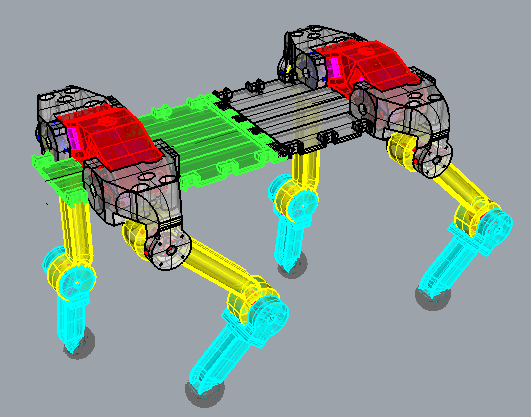
\includegraphics[width=.55\textwidth]{./Figuras/tetratopo.png}
\caption{Formato del robot propuesto.}
\label{fig:robotTetrapodo}
\end{figure}

En la Figura \ref{fig:robotDiagrama} se observan las relaciones entre los distintos componentes del sistema.

\begin{figure}[htpb]
\centering 
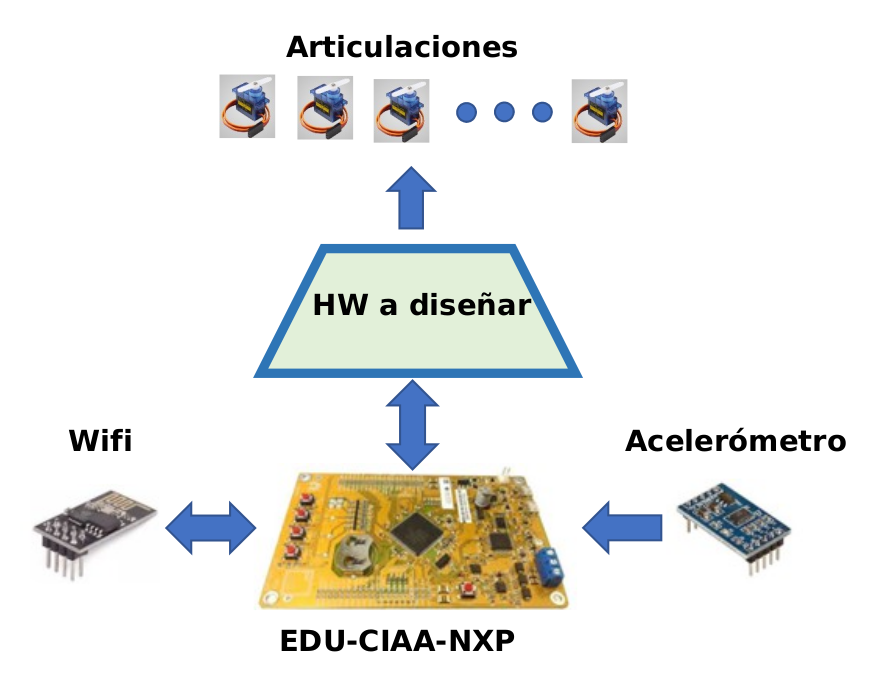
\includegraphics[width=.8\textwidth]{./Figuras/tetra.png}
\caption{Módulos de hardware del robot propuesto.}
\label{fig:robotDiagrama}
\end{figure}


\section{2. Identificación y análisis de los interesados}
\label{sec:interesados}

En esta plataforma se aplicarán algoritmos de Aprendizaje por Refuerzo (AR), se utilizara para formar recursos humanos dentro del Grupo de Inteligencia Artificial y Robótica (GIAR). Una vez afianzada la técnica, se realizará la transferencia de lo aprendido a los distintos clientes que posee el grupo de investigación, como materias afines de las distintas carreras de grado de la Universidad Tecnológica Nacional-Facultad Regional Buenos Aires.

\begin{table}[ht]
%\caption{Identificación de los interesados}
%\label{tab:interesados}
\begin{tabularx}{\linewidth}{@{}|l|X|X|l|@{}}
\hline
\rowcolor[HTML]{CCFFFF} 
Rol           & Nombre y Apellido & Organización 	& Puesto 	\\ \hline
%Auspiciante   & -  				& -					& -	   		\\ \hline
Cliente       & \clientename    &\empclientename	& -   		\\ \hline
Impulsor      & Lic. Patricia Cibeira    		&\empclientename 	& Secretario de SeCyT    		\\ \hline
Responsable   & \authorname     & FIUBA        		& Alumno 	\\ \hline
Colaboradores & Miembros del GIAR   & UTN-FRBA     		& -       	\\ \hline
Orientador    & \supname	    & \pertesupname 	& Director	trabajo final \\ \hline
%Equipo        & -          		& -             	& -        	\\ \hline
Opositores    & Otros Grupos Invest.    & UTN-FRBA             	& -        	\\ \hline
Usuario final & Alumnos de materia -IA     &\empclientename	& -        	\\ \hline
\end{tabularx}
\end{table}

%El Director suele ser uno de los Orientadores.
%No dejar celdas vacías; si no hay nada que poner en una celda colocar un signo ``-''.
%No dejar filas vacías; si no hay nada que poner en una fila entonces eliminarla.

%Sería deseable listar a continuación de la tabla las principales características de cada interesado.
 
%Por ejemplo:
%\begin{itemize}
%\item Auspiciante: es riguroso y exigente con la rendición de gastos. Tener mucho cuidado con esto.
%\item Equipo: Juan Perez, suele pedir licencia porque tiene un familiar con una enfermedad. Planificar considerando esto.
%\item Orientador: María Gómez, nos va a poder ayudar mucho con la gestión de impuestos.
%\end{itemize}

%\end{consigna}

\begin{itemize}
\item Orientador: Ing. Juan Carlos Gómez, posee mucha experiencia en el tema debido a su trabajo, y formación  profesional, pero no posee mucho tiempo.
\item Cliente: posee muchas restricciones con respecto a los costos.
\end{itemize}


\section{3. Propósito del proyecto}
\label{sec:proposito}

El propósito del proyecto es diseñar el hardware y el firmware de un controlador de movimientos para un robot tetrápodo de tres grados de libertad en cada extremo, y aplicar los conocimientos en materias de inteligencia artificial dictadas en la UTN-FRBA.


\section{4. Alcance del proyecto}
\label{sec:alcance}

El objetivo del proyecto comprende:

\begin{itemize}
\item Diseñar y armar el prototipo del hardware del robot tetrápodo.
\item Diseñar e implementar en la placa principal el software embebido de A.R.
\item Diseñar comandos para cambiar el modo de funcionaniento desde línea de comandos, desde una PC. 
\item Realizar el proyecto dentro del tiempo destinado al mismo.
\end{itemize}

El proyecto no incluye:

\begin{itemize}
\item Realizar pruebas de estructuras de hardware, para saber la vida útil del sistema.
\item Diseñar una interface gráfica amigable para cambiar los distintos modos de funcionamiento.
\item Diseñar y/o armar el cargador de baterías.
\item El diseño del módulo de alimentación se lo dejará para un estado posterior a este proyecto, como así también las pruebas de autonomía.

El objetivo del proyecto comprende:


\end{itemize}


\section{5. Supuestos del proyecto}
\label{sec:supuestos}

Se supone para el siguiente proyecto que:
\begin{itemize}
\item se posee el presupuesto para comprar todo lo relacionado con el hardware necesario para construir el robot. 
\item se contará con acceso a todo el equipamiento para la construcción y testeo de los distintos elementos electrónicos.
\item la complejidad de la programación se restringirá en función de las horas de trabajo propuestas para hacer este proyecto.
\item se podrá conseguir los distintos elementos electrónicos en este contexto de pandemia.
\end{itemize}

\section{6. Requerimientos}
\label{sec:requerimientos}

\begin{enumerate}
\item Requerimientos de funcionamiento general
	\begin{enumerate}
	\item El robot debe alimentarse mediante un sistema que le permita tener la posibilidad de desplazarse sin problemas.
	\item Se debe comunicar en forma inalámbrica y mediante el puerto USB de la placa principal. 
	\item El robot debe ser lo suficiente ligero para que los servomotores puedan mover las articulaciones.
	\end{enumerate}

\vspace{0.3cm} 

\item Grupo de requerimientos asociados con el hardware
	\begin{enumerate}
	\item El hardware debe ser fácilmente replicable utilizando una impresora 3D.
	\item Debe poseer la menor cantidad de piezas posibles, no mayor a cuarenta. 
	\item El cuerpo del robot debe albergar todo el hardware (motores, placa principal, drivers de motores, , etc.) necesario para el funcionamiento normal.
	\item Debe poseer un botón de parada de emergencia de fácil acceso, para interrumpir el funcionamiento del robot en caso de urgencia.
	\end{enumerate}
	
\vspace{0.3cm}	
	
\item Grupo de requerimientos asociados con el software
	\begin{enumerate}
	\item Se programará usando Lenguaje C, utilizando el modelo de capas.
	\item La herramienta de programación en Lenguaje C deberá poseer un modo DEBUG.
	\item El uso de memoria no debe exceder a la placa principal.
	\end{enumerate}
	
\vspace{0.3cm}
	
\item Requerimientos no funcionales
	\begin{enumerate}
	\item La estructura del robot no debe tener bordes filosos ni punzantes, que puedan ocasionar lesiones. 
	\item La velocidad que desarrolla el robot debe ser inferior a 1 m/seg.
	\end{enumerate}
	
\vspace{0.3cm}

\item Requerimientos documentación
	\begin{enumerate}
	\item Redactar el manual de uso. 
	\item Redactar un documento en donde se registre el código 
	fuente.
	\item Redactar un documento técnico que figuren los circuitos
	esquemáticos, y el armado de la plataforma.
	\end{enumerate}
\end{enumerate}

\vspace{2cm} 


\section{7. Historias de usuarios (\textit{Product backlog})}
\label{sec:backlog}

Criterio: a mayor valor de prioridad, la historia de usuario es más importante. Para el grado de ponderación se toma el criterio horas-hombre (valor de esfuerzo) que supone la implementación de la historia de usuario.

\begin{itemize}
\item Historia de usuario 1: Como docente quiero que el robot se pueda conectar a una red local, para poder controlarlo desde una posición remota.
	\begin{itemize}
	\item Prioridad : 1
	\item Ponderación : 5
	\end{itemize}
\item Historia de usuario 2: Como alumno quiero poder cambiar los distintos algoritmos de control, para poder sintonizar los movimientos de la plataforma móvil. 
	\begin{itemize}
	\item Prioridad : 2
	\item Ponderación : 5
	\end{itemize}	
\item Historia de usuario 3:  Como alumno quiero tener una aplicación  gráfica en un dispositivo móvil, para poder manejar los movimientos del robot mediante \textit{Wi-Fi} o el puerto USB. 
	\begin{itemize}
	\item Prioridad : 3
	\item Ponderación : 7
	\end{itemize}
\item Historia de usuario 4: Como ayudante de laboratorio encargado del robot quiero que se pueda reparar rápidamente, para no perder tiempo. 
	\begin{itemize}
	\item Prioridad : 4
	\item Ponderación : 3
	\end{itemize}	
\item Historia de usuario 5: Como docente quiero tener la posibilidad de contar con una fuente de energía a baterías para poder usar el robot en cualquier ambiente.
	\begin{itemize}
	\item Prioridad : 5
	\item Ponderación : 1
	\end{itemize}		
\end{itemize}

%\vspace{4cm} 

\section{8. Entregables principales del proyecto}
\label{sec:entregables}

Al final del proyecto se entregará: 
\begin{itemize}
\item Prototipo del robot.
\item Manual de uso.
\item Diagrama esquemático.
\item Código fuente.
\item Diagrama de instalación.
\item Informe final..
\end{itemize}


\section{9. Desglose del trabajo en tareas}
\label{sec:wbs}

\begin{enumerate}
\item Planificación de tareas. (40 hs)
	\begin{enumerate}
	\item Generación del documento de planificación del proyecto. (30 hs)
	\item Aprobación y revisión del documento de planificación del proyecto. (10 hs)
	\end{enumerate}
\item Investigación preliminar del hardware a utilizar. (38 hs)
	\begin{enumerate}
	\item Fabricación del robot. (20 hs)
	\item Placas electrónicas(placa principal, microcontrolador, drivers, etc). (10 hs)
	\item Características de los motores.  (4 hs)
	\item Características de las fuente de alimentación. (4 hs)
	\end{enumerate}
\item Selección y compra de los materiales del hardware. (8 hs)
	\begin{enumerate}
	\item Selección de los componentes. (5 hs)
	\item Compra y adquisición.(3 hs)
	\end{enumerate}
\item Armado y verificación de la estructura del robot. (43 hs)
	\begin{enumerate}
	\item Construcción de las piezas. (30 hs)
	\item Ensamblaje de piezas. (3 hs)
	\item Verificación de la estructura. (10 hs)
	\end{enumerate}
\item Armado y verificación de la electrónica del robot. (10 hs)
	\begin{enumerate}
	\item Armado de la placa adaptadora entre la placa principal y los distintos módulos. (5 hs)
	\item Cableado del robot. (2 hs)
	\item Verificación de la electrónica. (3 hs)
	\end{enumerate}	

%\vspace{4cm} 

\item Integración del hardware. (6 hs)	
\item Desarrollo del software (189hs)
	\begin{enumerate}
	\item Módulo PWM. (25 hs)
	\item Módulo Wi-Fi y protocolo de comunicaciones. (44 hs)
	\item Módulo acelerómetro.  (25 hs)
	\item Módulo de aprendizaje por refuerzo. (40 hs)
	\item Módulo manual. (25 hs)
	\item Integración de los distintos módulos. (30 hs)
	\end{enumerate}	
\item Verificación del software(\textit{Testing}). (75 hs)
	\begin{enumerate}
	\item Diseño de pruebas  de ensayo de los distintos módulos. (25 hs)
	\item Diseño de las distintas pruebas de navegación. (30 hs)
	\item Comparación de las distintas estrategias de navegación. (20 hs)
	\end{enumerate}	
\item Validación del sistema completo. (40 hs)
	\begin{enumerate}
	\item Ensayos de verificación del cliente en forma parcial. (20 hs)
	\item Ensayos de validación final. (20 hs)
	\end{enumerate}	
\item Presentación del trabajo. (151 hs)
	\begin{enumerate}
	\item Redacción de informes de avance. (10 hs)
	\item Redacción de manual de uso. (20 hs)
	\item Elaboración de circuitos esquemáticos. (20 hs)
	\item Redacción de memoria del proyecto. (80 hs)
	\item Preparación de la presentación pública del trabajo final. (20 hs)
	\item Presentación pública del trabajo final. (1 h)
	\end{enumerate}					
\end{enumerate}
Cantidad total de horas: (600 hs)

\pagebreak

\section{10. Diagrama de Activity On Node}
\label{sec:AoN}

En la figura \ref{fig:AoN}, se observa el camino crítico en color rojo. La unidad de tiempo definida en cada tarea es en hora.
 
\begin{figure}[htpb]
\centering 
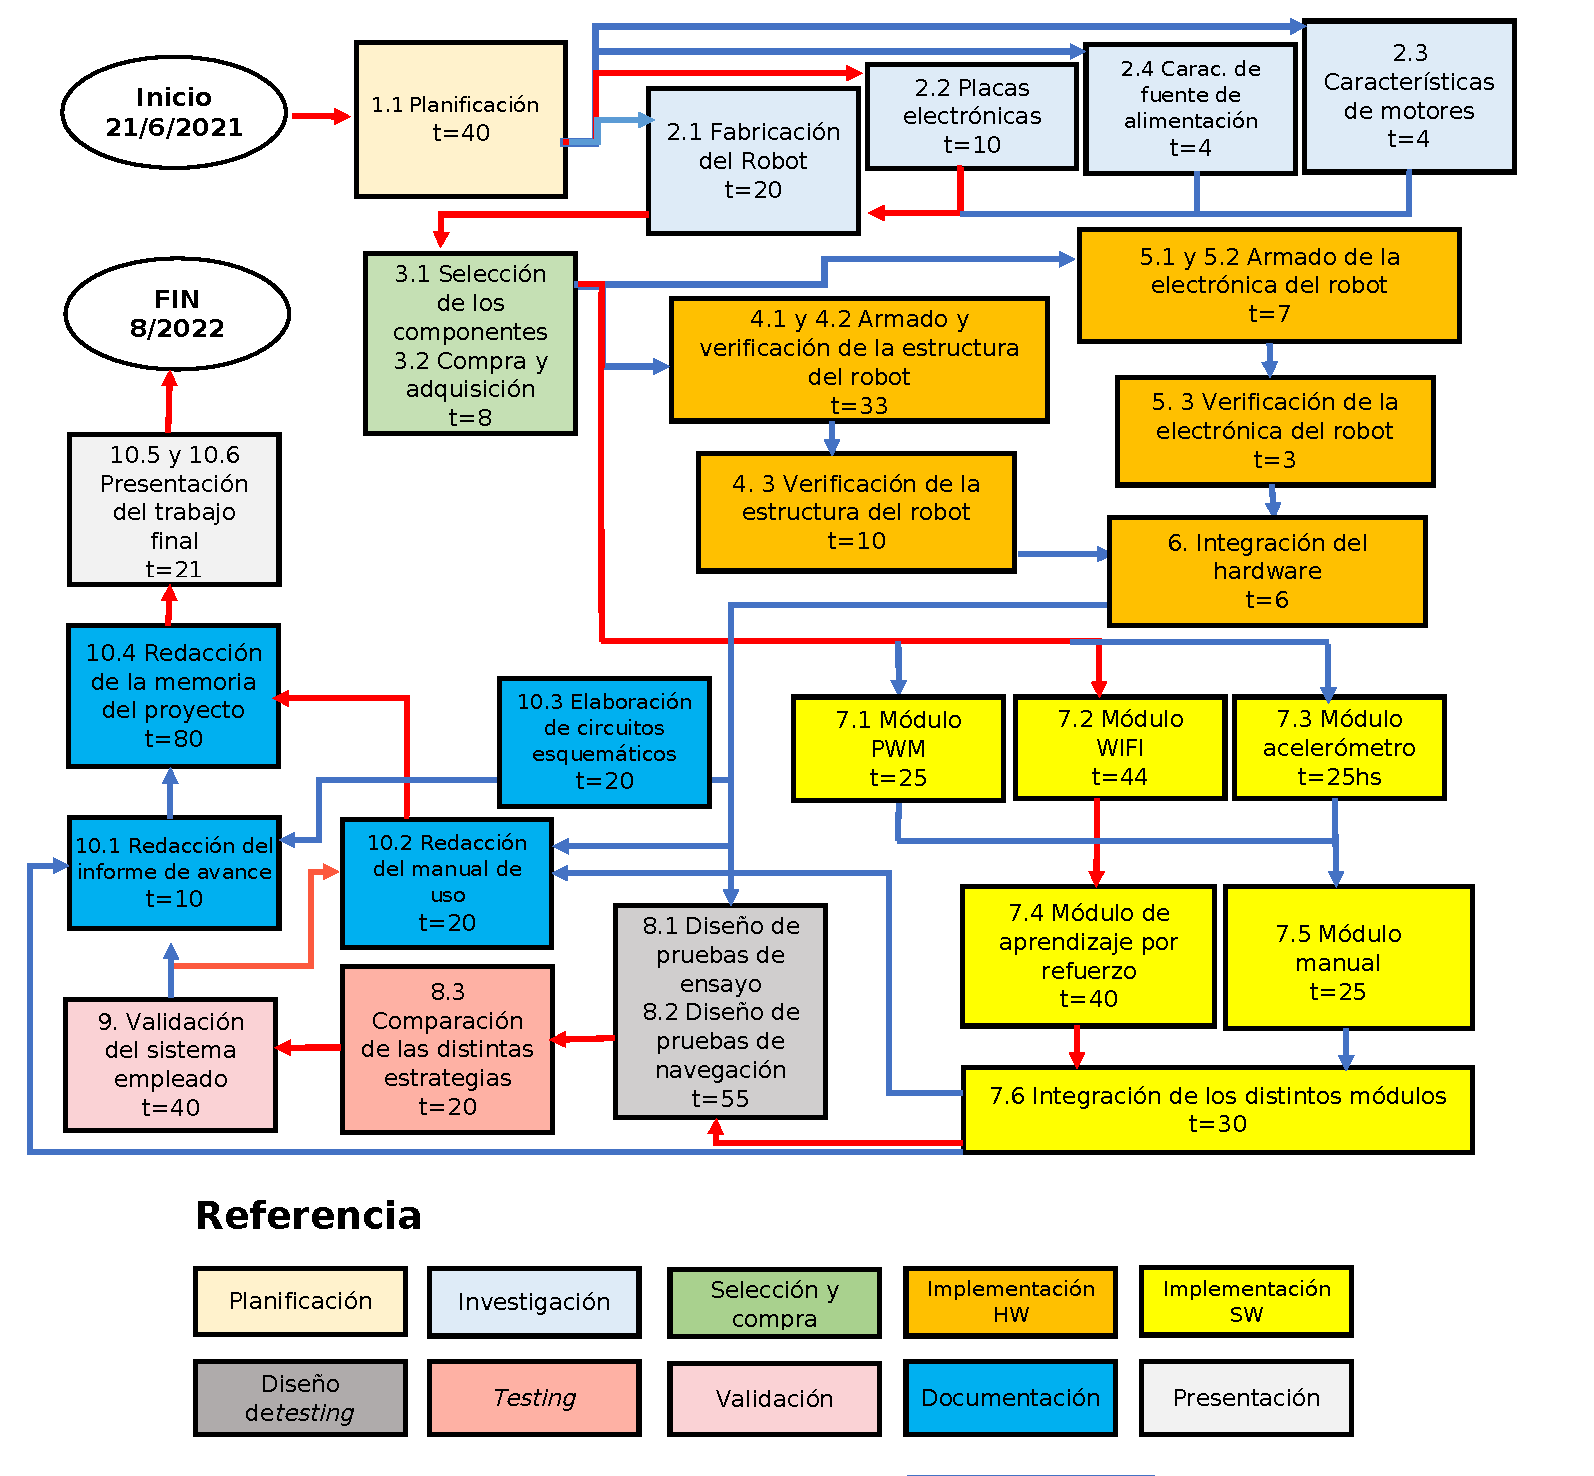
\includegraphics[width=\textwidth]{./Figuras/AoN.pdf}
\caption{Diagrama de \textit{Activity on Node}}
\label{fig:AoN}
\end{figure}

\vspace{4cm}

\section{11. Diagrama de Gantt}
\label{sec:gantt}

Los datos de la tabla 1 y de la figura 4 se obtuvieron de un software de gestión de proyectos teniendo en cuenta los días no laborables (feriados y vacaciones), y con una dedicación semanal de 10 horas reloj.

\begin{table}[htbp]
\centering
\resizebox{1\textwidth}{!}{
\begin{tabular}{|c|p{25em}|c|c|c|c|}
\hline
\textbf{Tarea}&{Nombre de tarea} & \textbf{Duración} & \textbf{Comienzo}& \textbf{Fin}&\textbf{Anterior}\\
\hline 1 & \textbf{Inicio} & 0 días & 21/06/21 & 21/06/21 &  \\
\hline 2 &\textbf{1. Planificación de tareas} & \textbf{20 días} & \textbf{21/06/21} & \textbf{16/07/21} &   \\
\hline 3 &1.1 Generación de documento & 30 horas & 21/06/21 & 09/07/21  & 1 \\
\hline 4 &1.2 Aprobación y revisión & 10 horas & 12/07/21 & 16/07/21  & 3 \\
\hline 5 &\textbf{2. Investigación preliminar del hardware} & \textbf{19 días} & \textbf{26/07/21} & \textbf{27/08/21} &   \\
\hline 6 & 2.1 Fabricación del Robot & 20 horas & 13/08/21 & 27/08/21 & 4,9,8,7 \\
\hline 7 & 2.2 Placas electrónicas & 10 horas & 26/07/21 & 06/08/21 & 4  \\
\hline 8 & 2.3 Características de motores & 4 horas & 09/08/21 & 10/08/21 & 7 \\
\hline 9 & 2.4 Características de baterías & 4 horas & 11/08/21 & 12/08/21 & 8 \\
\hline 10 & \textbf{3. Selección y compra de los materiales} & \textbf{4 días} & \textbf{30/08/21} & \textbf{02/08/21} &  \\
\hline 11 & 3.1 Selección de los componentes & 5 horas & 30/8/21 & 01/09/21 & 5 \\
\hline 12 & 3.2 Compra y adquisición & 3 horas & 01/09/21 & 02/09/21 & 11 \\
\hline 13 & \textbf{4. Armado y verificación de la estructura del robot} & \textbf{14 días} & \textbf{03/09/21} & \textbf{22/09/21} &  \\
\hline 14 & 4.1 Construcción de las piezas & 15 horas & 03/09/21 & 14/09/21 &  10 \\
\hline 15 & 4.2 Ensamblaje de las piezas & 3 horas & 14/09/21 & 15/09/21 & 14 \\
\hline 16 & 4.3 Verificación de la estructura & 10 horas & 16/09/21 & mié 22/09/21 & 15 \\
\hline 17 & \textbf{5. Armado y verificación de la electrónica del robot} & \textbf{5 días} & \textbf{03/09/21} & \textbf{09/09/21} &  \\
\hline 18 & 5.1 Armado de la placa principal & 5 horas & 03/9/21 & 07/09/21 & 10 \\
\hline 19 & 5.2 Cableado del robot & 2 horas & 07/09/21 & 08/09/21 & 18 \\
\hline 20 & 5.3 Verificación de la electrónica & 3 horas & 08/09/21 & 09/09/21 & 19 \\
\hline 21 & \textbf {6. Integración del hardware} & 2 horas & 23/09/21 & 23/09/21 & 13,17 \\
\hline 22 & \textbf{7. Desarrollo del software} & \textbf{55 días} & \textbf{03/09/21} & \textbf{23/09/21} &  \\
\hline 23 & 7.1 Módulo PWM & 25 horas & 03/09/21 & 21/09/21 & 10 \\
\hline 24 & 7.2 Módulo Wi-Fi & 40 horas & 03/09/21 & 30/09/21 & 10 \\
\hline 25 & 7.3 Módulo acelerómetro & 25 horas & 03/09/21 & 21/09/21 & 10 \\
\hline 26 & 7.4 Módulo de aprendizaje por refuerzo & 40 horas & 01/10/21 & 01/11/21 & 23,24,25  \\
\hline 27 & 7.5 Módulo manual & 25 horas & 01/10/21 & jue 21/10/21 & 23,24,25 \\
\hline 28 & 7.6 Integración de los distintos módulos & 30 horas & 02/11/21 & 23/11/21 & 26,27 \\
\hline 29 & \textbf{8. Verificación del software} & \textbf{37,5 días} & \textbf{24/11/21} & \textbf{16/02/22} &  \\
\hline 30 & 8.1 Diseño de pruebas de ensayo & 25 horas & 24/11/21 & 10/12/21 & 21,28 \\
\hline 31 & 8.2 Diseño de pruebas de navegación & 30 horas & mar 10/12/22 & 01/02/22 & 30 \\
\hline 32 & 8.3 Comparación de las distintas estrategias. & 20 horas & 01/02/22 & 16/02/22 & 31 \\
\hline 33 & \textbf{9. Validación del sistema empleado} & \textbf{20 días} & \textbf{16/02/22} & \textbf{18/03/22} &  \\
\hline 34 & 9.1 Ensayos de verificación del cliente parcial & 20 horas & 16/2/22 & 04/03/22 & 32 \\
\hline 35 & 9.2 Ensayos de validación final & 20 horas & 04/03/22 & 18/03/22 & 34 \\
\hline 36 & \textbf{10. Presentación del trabajo final} & \textbf{158 días} & \textbf{24/09/21} & \textbf{16/06/22} &  \\
\hline 37 & 10.1 Redacción del informe de avance & 10 horas & 18/03/22 & 28/03/22 & 28,33,39 \\
\hline 38 & 10.2 Redacción del manual de uso & 20 horas & 18/03/22 & 04/04/22 & 21,28,35 \\
\hline 39 & 10.3 Elaboración de los circuitos esquemáticos & 20 horas & 24/09/22 & 07/10/21 & 21 \\
\hline 40 & 10.4 Redacción de la memoria del proyecto & 80 horas & 04/04/22 & 02/06/22 & 37,38 \\
\hline 41 & 10.5 Preparación de la presentación pública & 20 horas & 02/06/22 & 16/06/22 & 40 \\
\hline 42 & 10.6 Presentación pública & 1 hora & 16/06/22 & 16/06/22 & 41 \\
\hline 43 & \textbf{Fin} & 0 días & 16/06/22 & 16/06/22 &  \\
\hline
\end{tabular}}
\caption{Inicio y fin de cada tarea}
\label{tab:CuadroGantt}
\end{table}

\newpage
\begin{landscape}
\begin{figure}[htpb]
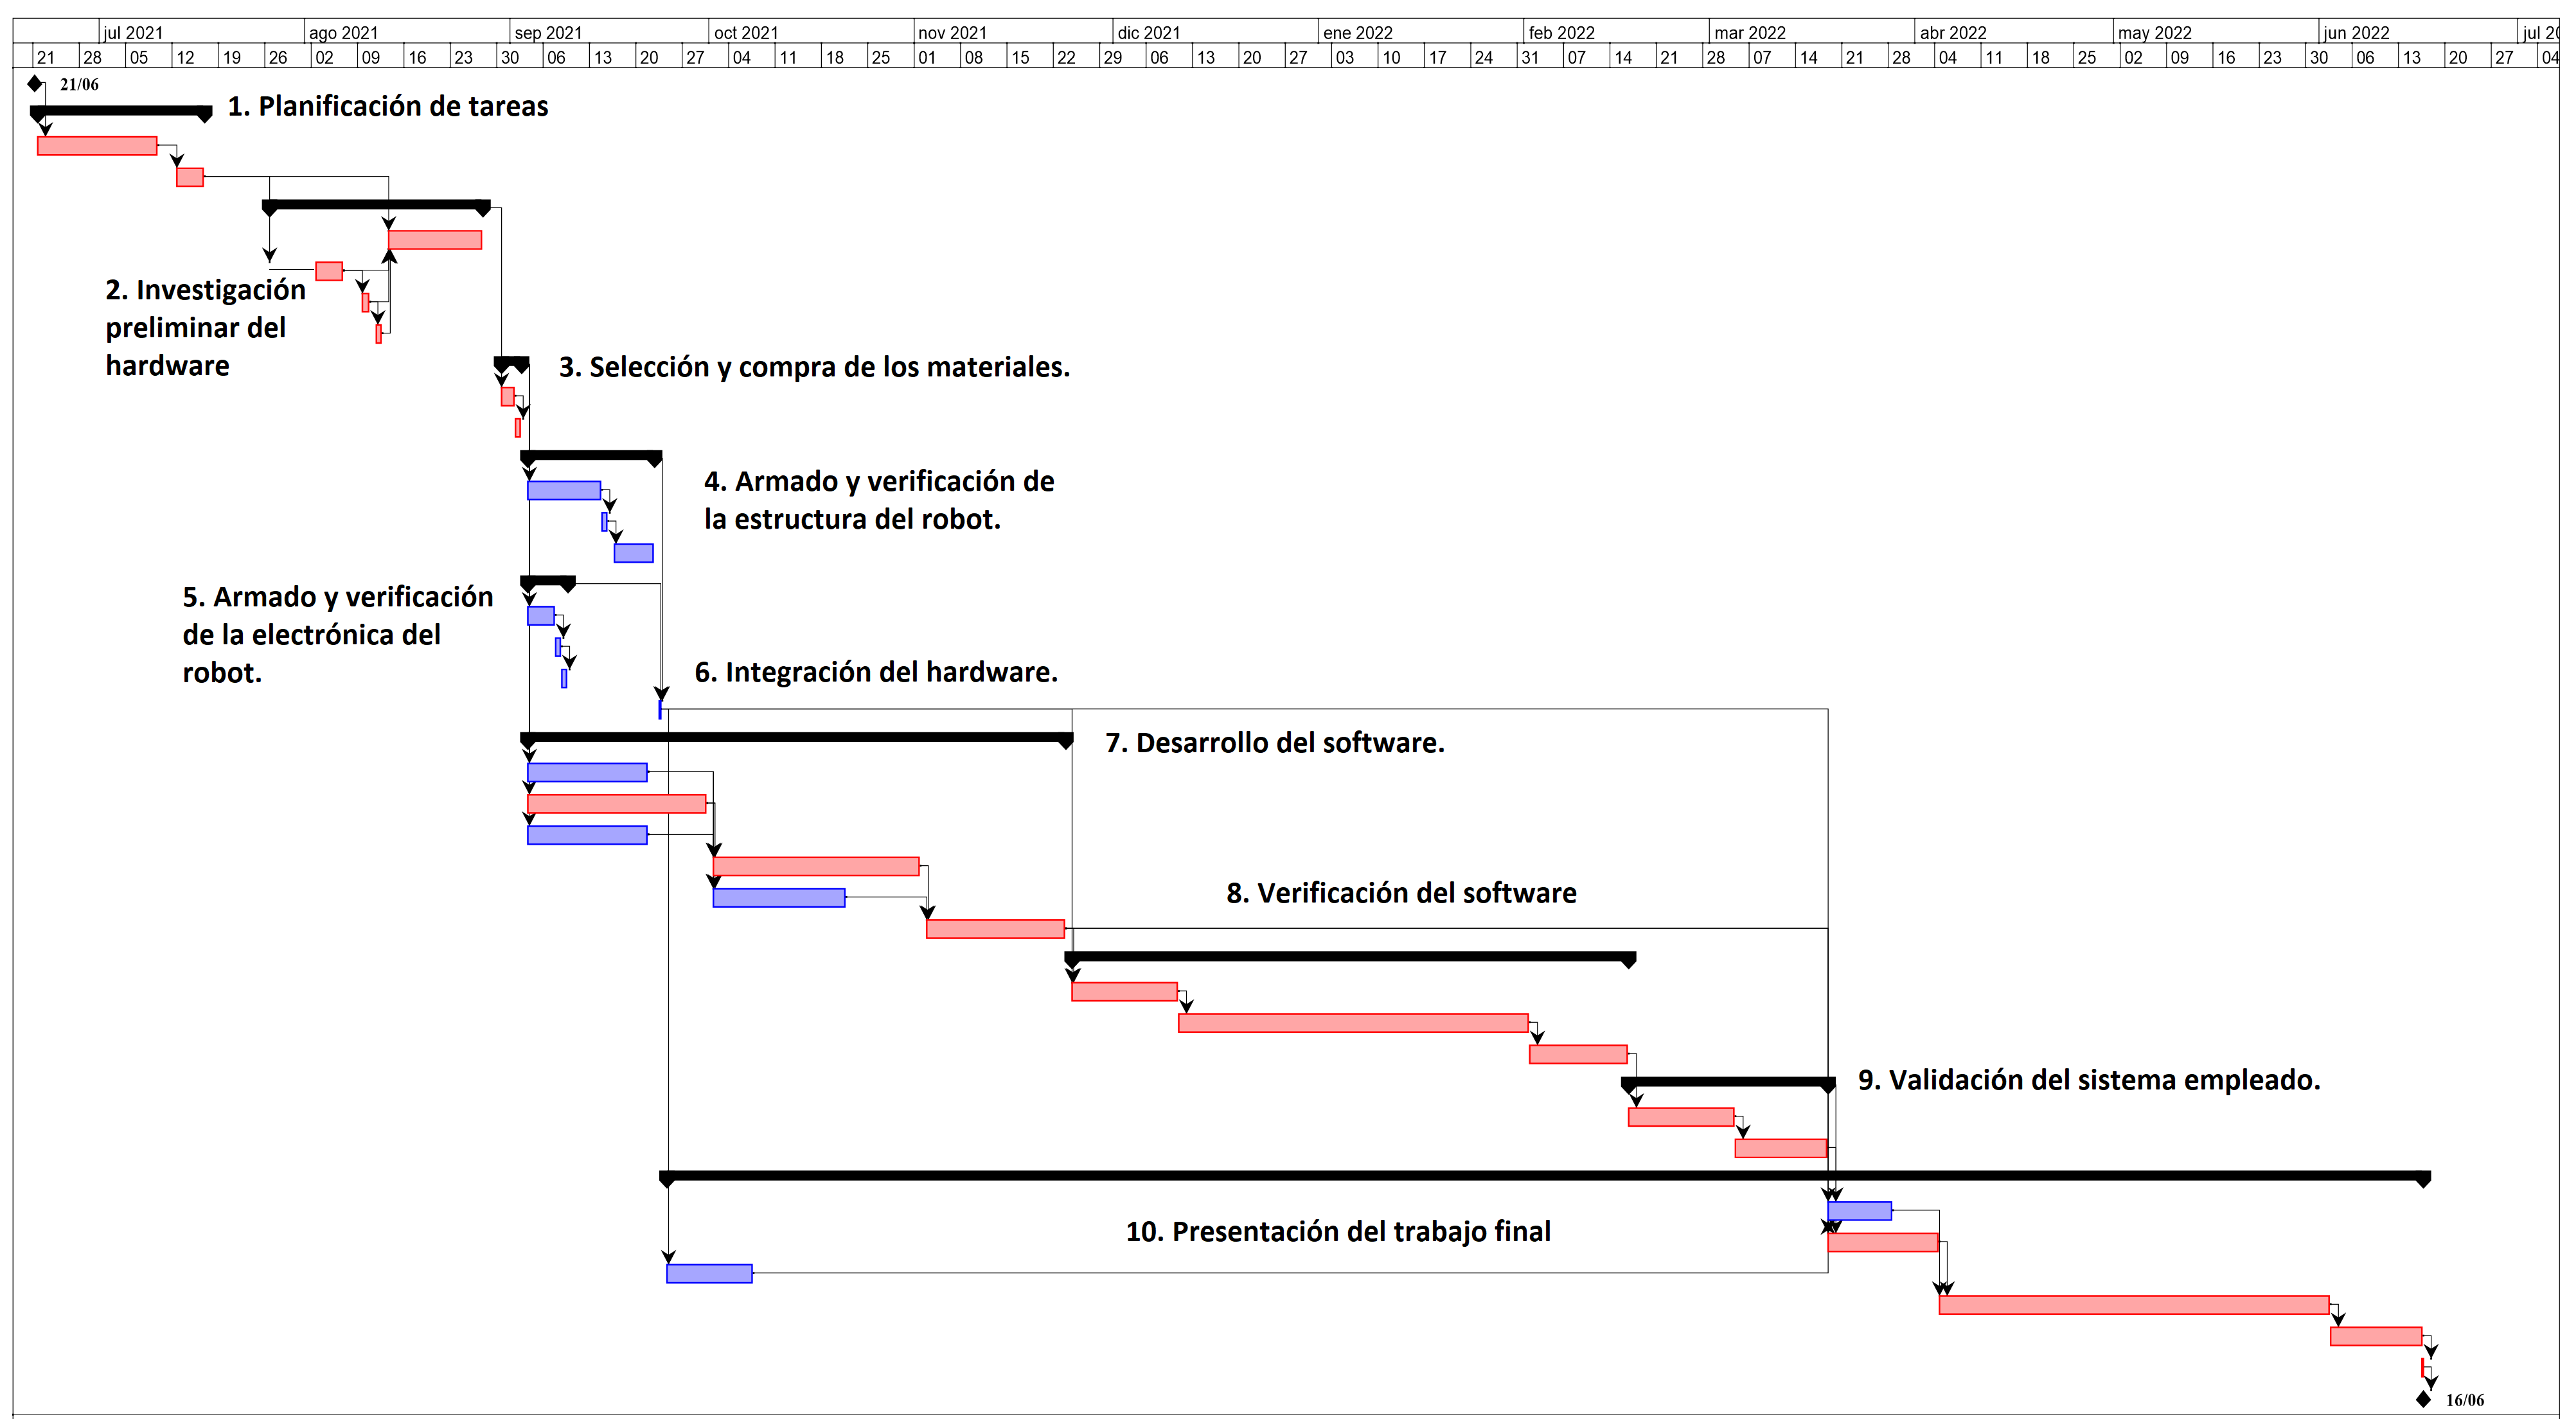
\includegraphics[width=1.6\textwidth]{./Figuras/gantt_tetrapodo_new.png}
\caption{Diagrama de \textit{Gantt}}
\label{fig:Gantt}
\end{figure}
\end{landscape}

\section{12. Presupuesto detallado del proyecto}
\label{sec:presupuesto}

\begin{table}[htpb]
\centering
\scalebox{1}[.9]{
\begin{tabularx}{\linewidth}{@{}|p{1em}|X|X|X|X|@{}}
\hline
\rowcolor[HTML]{C0C0C0} 
\multicolumn{5}{|c|}{\cellcolor[HTML]{CCFFFF}COSTOS DIRECTOS [\$]} \\ \hline
\rowcolor[HTML]{C0C0C0} 
\multicolumn{2}{|c|}{Descripción} &
  \multicolumn{1}{c|}{\cellcolor[HTML]{B0B0B0}Cantidad} &
  \multicolumn{1}{c|}{\cellcolor[HTML]{B0B0B0}Valor unitario} &
  \multicolumn{1}{c|}{\cellcolor[HTML]{B0B0B0}Valor total} \\ \cline{1-5}
\multirow{13}[1]{*}{\rotatebox{90}{Materiales}} & Driver doble puente H  (L298) &
  \multicolumn{1}{c|}{6} &
  \multicolumn{1}{c|}{550} &
  \multicolumn{1}{c|}{3.300} \\ \cline{2-5}
& Sermomotores de 5v tipo Futaba S3003&
   \multicolumn{1}{c|}{4} &
  \multicolumn{1}{c|}{700} &
  \multicolumn{1}{c|}{2.800} \\ \cline{2-5}
& Sermomotores de 5v tipo Sg90 &
   \multicolumn{1}{c|}{8} &
  \multicolumn{1}{c|}{310} &
  \multicolumn{1}{c|}{2.480} \\ \cline{2-5}  
& Placa principal(Beaglebone o similar) &
   \multicolumn{1}{c|}{1} &
  \multicolumn{1}{c|}{12.000} &
  \multicolumn{1}{c|}{12.000} \\ \cline{2-5}
& Porta baterías (4 pilas AA) &
  \multicolumn{1}{c|}{1} &
  \multicolumn{1}{c|}{1} &
  \multicolumn{1}{c|}{290} \\ \cline{2-5}
&  Baterias de Li-ion 3,7v 7800 mah&
   \multicolumn{1}{c|}{4} &
  \multicolumn{1}{c|}{400} &
  \multicolumn{1}{c|}{1.600} \\ \cline{2-5}
& Pulsador NA &
  \multicolumn{1}{c|}{1} &
  \multicolumn{1}{c|}{100} &
  \multicolumn{1}{c|}{100} \\ \cline{2-5}
& Placa  Wi-Fi(ESP1 8266)&
   \multicolumn{1}{c|}{1} &
  \multicolumn{1}{c|}{800} &
  \multicolumn{1}{c|}{800} \\ \cline{2-5} 
&  Placa acelerómetro (Mpu-9250)&
   \multicolumn{1}{c|}{1} &
  \multicolumn{1}{c|}{1.500} &
  \multicolumn{1}{c|}{1.500} \\ \cline{2-5}
&  Cables varios &
  \multicolumn{1}{c|}{1} &
  \multicolumn{1}{c|}{1} &
  \multicolumn{1}{c|}{500} \\ \cline{2-5}
&  Conectores varios &
  \multicolumn{1}{c|}{1} &
  \multicolumn{1}{c|}{1} &
  \multicolumn{1}{c|}{800} \\ \cline{2-5}
&  Placa experimental 20x20 cm &
  \multicolumn{1}{c|}{1} &
  \multicolumn{1}{c|}{400} &
  \multicolumn{1}{c|}{400} \\ \cline{2-5}
&  Estaño 60/40 0,8mm 3m&
  \multicolumn{1}{c|}{1} &
  \multicolumn{1}{c|}{250} &
  \multicolumn{1}{c|}{250} \\ \cline{2-5} 
&  Filamento 1,75 mm (PLA) &
  \multicolumn{1}{c|}{1} &
  \multicolumn{1}{c|}{1.600} &
  \multicolumn{1}{c|}{1.600} \\ \cline{2-5}  
  
\multicolumn{4}{|c|}{Mano de obra} &
  \multicolumn{1}{c|}{150.000} \\ \hline 
  
\multicolumn{4}{|c|}{SUBTOTAL} &
  \multicolumn{1}{c|}{178.420} \\ \hline
\rowcolor[HTML]{C0C0C0} 
\multicolumn{5}{|c|}{\cellcolor[HTML]{CCFFFF}COSTOS INDIRECTOS [\$]} \\ \hline
\rowcolor[HTML]{C0C0C0} 
\multicolumn{4}{|c|}{Descripción} &
  \multicolumn{1}{c|}{\cellcolor[HTML]{B0B0B0}Valor total} \\ \hline
\multicolumn{4}{|c|}{30\% de los costos directos} &
  \multicolumn{1}{c|}{53.526} \\ \hline
  
\multicolumn{4}{|c|}{SUBTOTAL [\$]} &
  \multicolumn{1}{c|}{53.526} \\ \hline
\multicolumn{4}{|c|}{\cellcolor[HTML]{B0B0B0}TOTAL [\$]} &
  \multicolumn{1}{c|}{\cellcolor[HTML]{B0B0B0}285.472} \\ \hline   
\end{tabularx}
}
\caption{Presupuesto}
\label{tab:Presupuesto}
\end{table}


Aclaración: el presupuesto de la tabla \ref{tab:Presupuesto} se realizó con fecha 03/08/2021 en pesos argentinos (\$). La  cotización es de \$175 por dólar estadounidense (u\$s). El costo total es \$285.472 o su equivalente en u\$s1.632.

\vspace{40em}



\section{13. Gestión de riesgos}
\label{sec:riesgos}
a) Identificación de los riesgos: 
\renewcommand{\tabularxcolumn}[1]{>{\arraybackslash}m{#1}}
\begin{table}[htpb]
\centering
\scalebox{1}[.9]{
\begin{tabularx}{\textwidth}{@{}|c|p{1em}|m{4em}|c|X|@{}}
\hline
\multicolumn{1}{|c|}{\cellcolor[HTML]{CCFFFF}Nro.} &
\multicolumn{1}{|c|}{\cellcolor[HTML]{CCFFFF}Descripción del riesgo} &
\multicolumn{1}{|c|}{\cellcolor[HTML]{CCFFFF}\begin{tabular}{m{4em}}Severidad \\ Ocurrencia \end{tabular} } &
\multicolumn{1}{|c|}{\cellcolor[HTML]{CCFFFF}Valor}&
\multicolumn{1}{|c|}{\cellcolor[HTML]{CCFFFF} Justificación}\\ \hline

\multirow{2}{*}{1}  							&
	\multirow{2}{*}{\begin{tabular}{c}
	Pérdida/Destrucción \\
	del kit de desarrollo \end{tabular}}		&
	Severidad 									&
	10											&
	El daño en el kit de desarrollo modifica en 
	numerosas etapas del desarrollo de este 
	proyecto. Como por ejemplo no poder probar
	el software, no terminar de construir el
	prototipo, etc. \\ \cline{3-5}
	& &
	Ocurrencia 									&
	5											&
	La posibilidad de que suceda es moderada, ya 
	que el kit se montará en una plataforma móvil.
	\\ \hline
\multirow{2}{*}{2}  							&
	\multirow{2}{*}{\begin{tabular}{c}
	Destrucción del \\
	driver de motor \\
	(L298) \end{tabular}}		&
	Severidad 									&
	7											&
	El daño en el driver atrasaría algunas tareas,
	pero otras  podrían continuar.  \\ \cline{3-5}
	& &
	Ocurrencia 									&
	6											&
	Si el motor se bloquea, por el driver puede 
	circular mucha corriente y se puede quemar.
	\\ \hline

\multirow{2}{*}{3}  							&
	\multirow{2}{*}{\begin{tabular}{c}
	Falta de tiempo  \\
	para adquirir los  \\
	conocimientos para \\
	implementar el\\
	software de AR.  
	\end{tabular}}								&
	Severidad 									&
	6											&
	El algoritmo se está probando en otra plataforma
	pero de características muy distintas.  \\ \cline{3-5}
	& &
	Ocurrencia 									&
	3											&
	La probabilidad es baja, ya que se puede adaptar
	distintos niveles de complejidad.
	\\ \hline

\multirow{2}{*}{4}  							&
	\multirow{2}{*}{\begin{tabular}{c}
	\\
	Daños en la \\ 
	impresora 3D.  \end{tabular}}				&
	Severidad 									&
	6											&
	Se usa para fabricar las piezas del robot en
	un etapa temprana el proyecto. \\ \cline{3-5}
	& &
	Ocurrencia 									&
	7											&
	La probabilidad es alta, ya que su funcionamiento depende
	de muchos factores (que los inyectores no se tapen, que las
	tensiones de las correas sean las correctas, que no se
	quemen los drivers de los motores, que el firmware
	no se dañe, etc ).	\\ \hline
	
\multirow{2}{*}{5}  							&
	\multirow{2}{*}{\begin{tabular}{c}
	Capacidad o poten-\\
	cia  del pack de bate-\\
	ría insuficiente para\\
	cumplir con los reque-\\
	rimientos planteados\\
	\end{tabular}}								&
	Severidad 									&
	6											&
	Se usan baterías Li-ion, algunos consumos pueden
	ser vitales para el éxito del proyecto. \\ \cline{3-5}
	& &
	Ocurrencia 									&
	7											&
	La probabilidad es alta, no se tiene experiencia en el 
	manejo de este tipo de batería.	\\ \hline	
	
\multirow{2}{*}{6}  							&
	\multirow{2}{*}{\begin{tabular}{c}
	Daño en la computa-\\ 
	dora que se usa para \\
 	programar y docu- \\
	mentar el proyecto.
	\end{tabular}}								&
	Severidad 									&
	7											&
	Se usa para el diseño de las piezas del robot,
	programar los algoritmos en la placa princial,
	y la documentación del proyecto. \\ \cline{3-5}
	& &
	Ocurrencia 									&
	5											&
	No es una computadora moderna, su probabilidad de falla es 
	moderada.	\\ \hline	
	
\end{tabularx}
}
\caption{Gestión de riesgos}
\label{tab:GestionRiesgos}
\end{table}

La ``severidad'' y la ``probabilidad de ocurrencia'' se califican de 1 a 10, siendo el número más alto correspondiente a la mayor severidad o la mayor probabilidad.
\vspace{5em}

%\begin{consigna}{red}
%a) Identificación de los riesgos (al menos cinco) y estimación %de sus consecuencias: 
%Riesgo 1: detallar el riesgo (riesgo es algo que si ocurre %altera los planes previstos)
%\begin{itemize}
%\item Severidad (S): mientras más severo, más alto es el número %(usar números del 1 al 10).\\
%Justificar el motivo por el cual se asigna determinado número de %severidad (S).
%\item Probabilidad de ocurrencia (O): mientras más probable, más %alto es el número (usar del 1 al 10).\\
%Justificar el motivo por el cual se asigna determinado número de %(O). 
%\end{itemize}   

%Riesgo 2:
%\begin{itemize}
%\item Severidad (S): 
%\item Ocurrencia (O):
%\end{itemize}

%Riesgo 3:
%\begin{itemize}
%\item Severidad (S): 
%\item Ocurrencia (O):
%\end{itemize}

b) Tabla de gestión de riesgos: (El RPN se calcula como \%RPN=SxO)

\begin{table}[htpb]
\centering
\begin{tabular}{@{}|c|c|c|c|c|c|c|@{}}
\hline
\rowcolor[HTML]{CCFFFF} 
\cellcolor[HTML]{CCFFFF}Nº de Riesgo & \cellcolor[HTML]{CCFFFF}S & \cellcolor[HTML]{CCFFFF}O & \cellcolor[HTML]{CCFFFF}RPN & \cellcolor[HTML]{CCFFFF}S* & \cellcolor[HTML]{CCFFFF}O* & \cellcolor[HTML]{CCFFFF}RPN* \\ \hline
 1	& 10 & 5 & \cellcolor{red} 50 & 5 & 5 & \cellcolor{green}25     \\ \hline
 2	&  7 & 6 & \cellcolor{red}42 & 3 & 5 & \cellcolor{green}15     \\ \hline
 3	&  6 & 3 & \cellcolor{green}18 &    &    &      \\ \hline
 4	&  6 & 7 & \cellcolor{red}42 & 6 & 3 & \cellcolor{green}18     \\ \hline
 5  &  6 & 7 & \cellcolor{red}42 & 3 & 5 & \cellcolor{green}15     \\ \hline
 6  &  7 & 5 & \cellcolor{green}35 &    &    &      \\ \hline
\end{tabular}%
\caption{RPN}
\label{tab:RPN}
\end{table}

\textbf{Criterio adoptado}: se tomarán medidas de mitigación de los riesgos cuyos RPN sean mayores a 40.

\textbf{Aclaración}: en la tabla \ref{tab:RPN} los valores marcados con (*) corresponden luego de haber aplicado el plan de mitigación de riesgos.

%\begin{consigna}{red}
%b) Tabla de gestión de riesgos:      (El RPN se calcula como %RPN=SxO)

%\begin{table}[htpb]
%\centering
%\begin{tabularx}{\linewidth}{@{}|X|c|c|c|c|c|c|@{}}
%\hline
%\rowcolor[HTML]{C0C0C0} 
%Riesgo & S & O & RPN & S* & O* & RPN* \\ \hline
%       &   &   &     &    &    &      \\ \hline
%       &   &   &     &    &    &      \\ \hline
%       &   &   &     &    &    &      \\ \hline
%       &   &   &     &    &    &      \\ \hline
%       &   &   &     &    &    &      \\ \hline
%\end{tabularx}%
%\end{table}

%Criterio adoptado: 
%Se tomarán medidas de mitigación en los riesgos cuyos números de %RPN sean mayores a ....

%Nota: los valores marcados con (*) en la tabla corresponden %luego de haber aplicado la mitigación.

\vspace{0.5cm}

c) Plan de mitigación de los riesgos que originalmente excedían el RPN máximo establecido:
 
\begin{itemize}
\item Riesgo 1: Pérdida/Destrucción	del kit de desarrollo.
	Medidas de mitigación: Para minimizar este riesgo se prevee una partida presupuestaria para comprar otra placa en caso de que sea necesario. Se habla con el proveedor y asegura tener \textit{stock} para los próximos meses y un plazo de entrega no mayor a 24 horas.
	\begin{itemize}
	\item Severidad(S): 5 Disminuye la severidad, algunas tareas pueden tener un retraso no significativo. 
	\item  Probabilidad de ocurrencia(O): 5 La probabilidad de ocurrencia no cambia debido al escaso conocimiento de la placa principal. 
	\end{itemize}
\item Riesgo 2:  Falta de tiempo para adquirir los conocimientos
para implementar el software de AR.
	Medidas de mitigación: El firmware de la placa en un primer prototipo puede salir con una versión acotada, al proyecto estaría aprobado por el cliente con el módulo del PID clásico y una de las técnicas de aprendizaje por refuerzo. Se puede recurrir al asesoramiento de expertos en el tema.
	\begin{itemize}
	\item Severidad(S): 3 La severidad disminuye considerablemente, se tiene la posibilidad de tener otras fuentes de información.
	\item  Probabilidad de ocurrencia(O): 5 Probabilidad de ocurrencia media, hay que ver la disponibilidad de los horarios de los expertos en el tema para ver si pueden atender nuestras consultas.  
	\end{itemize} 
\item Riesgo 4: Daños en la	impresora 3D.
	Medidas de mitigación: Se debe tener en \textit{stock} los repuestos necesarios para reemplazar en caso de ser necesarios. Los repuestos como la boquilla fusora, y las correas dentadas no son caras y se consiguen en el mercado.
	\begin{itemize}
	\item Severidad(S): 6 La severidad no cambia, la impresión de las piezas es un punto critico.
	\item  Probabilidad de ocurrencia(O): 3 Disminuye considerablemente, ya que al tener los repuestos se puede prevenir que no deje de funcionar. Hay algunos repuestos como la placa de control que son difíciles de conseguir, en tal caso hay que recurrir a otro tipo de estrategia de mitigación
	\end{itemize}
\item Riesgo 5: Capacidad o potencia del pack de batería	insuficiente para cumplir con los requerimientos planteados.
	Medidas de mitigación: Se debe diseñar el pack de batería para tener la posibilidad o de ampliar la capacidad de \textit{mAh} de las baterías de \textit{Li-ion}, o cambiarlas por otra tecnología como de \textit{NiCd} o \textit{NiMH}. Por tal motivo en el diseño se adoptó el uso de baterías de formato AA o tipo 14500.
	\begin{itemize}
	\item Severidad(S): 3 Disminuye considerablemente al tener varias alternativas.
	\item  Probabilidad de ocurrencia(O): 5 La probabilidad de ocurrencia es media, ya que de algunas baterías se carece del conocimiento de funcionamiento detallado. 
	\end{itemize}
\end{itemize}


\section{14. Gestión de la calidad}
\label{sec:calidad}

1. Requerimientos de funcionamiento general.
\begin{itemize} 
\item Req \#1.1: El robot debe alimentarse mediante un sistema que le permita tener la posibilidad de desplazarse sin problemas.
\begin{itemize}
\item Verificación y validación:
	\begin{itemize}
	\item Verificación para confirmar si se cumplió con lo requerido 	antes de mostrar el sistema al cliente:\\
	Se verifican los consumos de todas las placas del sistema 				mediante las hojas de datos y mediciones empíricas. Se hacen los 	cálculos de consumos y se registra la autonomía del robot en 			condiciones normales de funcionamiento. Con la batería al 100\%
	 de carga, se hace mover al robot en por lo menos en dos direcciones en una circunferencia de 1 metro de diámetro.
	\item Validación con el cliente para confirmar que está de 				acuerdo en que se cumplió con lo requerido:\\
	Con la batería completa se hará mover al robot en tres distancias sugeridas por el cliente de no más de 1 metro de largo, para validad 	este requerimiento.
	\end{itemize}
\end{itemize}	
\end{itemize}

\begin{itemize} 
\item Req \#1.2: Se debe comunicar en forma inalámbrica.
\begin{itemize} 
\item Verificación y validación:
	\begin{itemize}
	\item Verificación para confirmar si se cumplió con lo requerido 	antes de mostrar el sistema al cliente:\\
	Se verificarán las hojas de datos del módulo inalámbrico, 
	distancia de comunicación, velocidad de comunicación, potencia
	de transmisión, etc. Se verificará con el depurador de programa
	(\textit{debugger}) que al mandar tramas no válidas o con errores 
	de secuencia, el robot no las ejecute.
	\item Validación con el cliente para confirmar que está de 				acuerdo en que se cumplió con lo requerido:\\
	Mediante una prueba empírica se le envía comandos de movimiento
	al robot (hacia adelante, hacia atrás, giro a la derecha e
	izquierda), para demostrar que la plataforma móvil responde.
\end{itemize}
	
	\end{itemize}
\end{itemize}

\vspace{1cm}

\begin{itemize} 
\item Req \#1.3: El robot debe ser lo suficiente ligero para que los servomotores puedan mover las articulaciones.
\begin{itemize} 
\item Verificación y validación:
	\begin{itemize}
	\item Verificación para confirmar si se cumplió con lo requerido 	antes de mostrar el sistema al cliente:\\
	Se realiza los cálculos de torque de cada servomotor, con las peores condiciones de peso.  
	\item Validación con el cliente para confirmar que está de 				acuerdo en que se cumplió con lo requerido:\\
	Se hacen mover cada articulación en un ángulo de más o menos 45º de su posición de reposo, verificando mediante mediciones el cumplimiento de cada una de ellas.  
	\end{itemize}
\end{itemize}
\end{itemize}


2. Grupo de requerimientos asociados con el hardware.

\begin{itemize}
\item Req \#2.1: El hardware debe ser fácilmente replicable utilizando una impresora 3D.
\begin{itemize}
\item Verificación y validación:
	\begin{itemize}
	\item Verificación para confirmar si se cumplió con lo requerido 	antes de mostrar el sistema al cliente:\\
	Se verifican que todos los elementos estructurales del
 	robot puedan realizarse por una impresora 3D con un solo 
 	extrusor, eso significa que no se necesite por ejemplo de
 	material de soporte	especiales, que las dimensiones sean
 	menores que una cama de impresión estándar (20x20 cm), 
 	que el filamento sea fácil de conseguir (PLA o ABS), etc.
	\item Validación con el cliente para confirmar que está de 				acuerdo en que se cumplió con lo requerido:\\
	Se muestran los planos de donde se obtuvieron las impresiones de 
	los componentes  que conforman la plataforma.    
	\end{itemize}
\end{itemize}
\end{itemize}

\begin{itemize}
\item Req \#2.2: Debe poseer la menor cantidad de piezas posibles, no mayor a cuarenta. utilizando una impresora 3D.
\begin{itemize}
\item Verificación y validación:
	\begin{itemize}
	\item Verificación para confirmar si se cumplió con lo requerido 	antes de mostrar el sistema al cliente:\\
	Se hace un listado detallado de todos los componentes
	estructurales del hardware y se verifican que la cantidad sea 
	menor a la del requerimiento.
	\item Validación con el cliente para confirmar que está de 				acuerdo en que se cumplió con lo requerido:\\
	Se muestra al cliente el listado detallado elaborado en la
	 prueba de verificación. 
	\end{itemize}
\end{itemize}
\end{itemize}

\begin{itemize}
\item Req \#2.3: El cuerpo del robot debe albergar todo el hardware (motores, placa EDU-CIAA, drivers de motores, baterías, etc.) necesario para el funcionamiento normal.
\begin{itemize}
\item Verificación y validación:
	\begin{itemize}
	\item Verificación para confirmar si se cumplió con lo requerido 	antes de mostrar el sistema al cliente:\\
	Mediante planos se verifica que todos los elementos
	estructurales del robot, las distintas placas, los motores, y
	sensores se encuentran autocontenidos.  
	\item Validación con el cliente para confirmar que está de 				acuerdo en que se cumplió con lo requerido:\\
	Se demuestra al cliente empíricamente se cumple este requisito.
	\end{itemize}
\end{itemize}
\end{itemize}

\begin{itemize}
\item Req \#2.4: Debe poseer un botón de parada de emergencia de fácil acceso, para interrumpir el funcionamiento del robot en caso de urgencia.
\begin{itemize}
\item Verificación y validación:
	\begin{itemize}
	\item Verificación para confirmar si se cumplió con lo requerido 	antes de mostrar el sistema al cliente:\\
	Se depura el programa  y verifica que sin importar en que
	secuencia de programa se encuentre el software, al pulsar el
	botón se invoca la rutina de parada.  
	\item Validación con el cliente para confirmar que está de 				acuerdo en que se cumplió con lo requerido:\\
	Se hace funcionar al robot en una  trayectoria circular, y se
	verifica que cuando se presiona el botón de parada cumple este
	requerimiento.  
	\end{itemize}
\end{itemize}
\end{itemize}

3. Grupo de requerimientos asociados con el software.

\begin{itemize}
\item Req \#3.1: Se programará usando Lenguaje C, utilizando el modelo de capas.
\begin{itemize}
\item Verificación y validación:
	\begin{itemize}
	\item Verificación para confirmar si se cumplió con lo requerido 	antes de mostrar el sistema al cliente:\\
	Se analizarán las hojas de datos de la placa principal  y se
	verificará que usando un ambiente de programación en Lenguaje C
	se pueda programar la placa. Se controlará que todo el código
	fuente utilizado para programar al producto final esté escrito
	en Lenguaje C y con llamadas a las sAPI.
	Se generará un documento en donde se registren todas las rutinas
	que conforman el proyecto. 
	\item Validación con el cliente para confirmar que está de 				acuerdo en que se cumplió con lo requerido:\\
	Se presentará el informe del listado del código fuente con las
	rutinas que conforman el proyecto.   
	\end{itemize}
\end{itemize}
\end{itemize}

\begin{itemize}
\item Req \#3.2: La herramienta de programación en Lenguaje C deberá poseer un modo DEBUG.
\begin{itemize}
\item Verificación y validación:
	\begin{itemize}
	\item Verificación para confirmar si se cumplió con lo requerido 	antes de mostrar el sistema al cliente:\\
	Se verificará de las hojas de datos de la placa de desarrollo
	que posea un puerto serie extra, o algún otro método que permita tener información de depuración. 
	\item Validación con el cliente para confirmar que está de 				acuerdo en que se cumplió con lo requerido:\\
	Se configurará el prototipo para que envíe información de depuración a través de algún medio de comunicación con el cliente.
	\end{itemize}
\end{itemize}
\end{itemize}

\begin{itemize}
\item Req \#3.3: El uso de memoria no debe exceder a la placa principal.
\begin{itemize}
\item Verificación y validación:
	\begin{itemize}
	\item Verificación para confirmar si se cumplió con lo requerido 	antes de mostrar el sistema al cliente:\\
	Se analizará las hojas de datos de la placa de control y de su
	microprocesador para que con el código generado en el proyecto cumpla con este requerimiento.
	\item Validación con el cliente para confirmar que está de 				acuerdo en que se cumplió con lo requerido:\\
	Se compilará y  un programa de prueba en la placa de
 	desarrollo para validar el requerimiento.
	\end{itemize}
\end{itemize}
\end{itemize}

\vspace{0.5cm}

4. Requerimientos no funcionales

\begin{itemize}
\item Req \#4.1: La estructura del robot no debe tener bordes filosos ni punzantes, que puedan ocasionar lesiones. 
\begin{itemize}
\item Verificación y validación:
	\begin{itemize}
	\item Verificación para confirmar si se cumplió con lo requerido 	antes de mostrar el sistema al cliente:\\
	Se verificará con los planos estructurales de las piezas del
	robot, que todos los bordes externos si terminan en una arista,
	no sean ángulos inferiores a 90 grados, o que sean redondeados
	con un diámetro mayor a 0,5 mm. Se generará un informe
	detallando.
	\item Validación con el cliente para confirmar que está de 				acuerdo en que se cumplió con lo requerido:\\
	Se presentará el informe generado en la validación, constatando  
	físicamente las terminaciones de los bordes externos del robot.
	\end{itemize}
\end{itemize}
\end{itemize}

\begin{itemize}
\item Req \#4.2: La velocidad que desarrolla el robot debe ser inferior a 1 m/seg. 
\begin{itemize}
\item Verificación y validación:
	\begin{itemize}
	\item Verificación para confirmar si se cumplió con lo requerido 	antes de mostrar el sistema al cliente:\\
 	Con las hojas de datos de los servomotores, calculando la máxima elongación de cada articulación y el tiempo de respuesta, se calcula la velocidad máxima. sta velocidad debe ser menor a la del requerimiento.
	\item Validación con el cliente para confirmar que está de 				acuerdo en que se cumplió con lo requerido:\\
	Se medirá la velocidad que alcanza el robot a máxima carga de
	batería con un método indirecto. Se pondrán a 5 metros de
	distancia en línea recta dos marcas en un piso plano y liso. El
	robot se pondrá en posición de reposo a un metro atrás de la
	primera marca y se acelerará logrando tener la mayor zancada de paso en cada extremidad en el menor tiempo posible. Se medirá el
	tiempo en que tarda en cruzar las dos marcas, calculando así su
	velocidad máxima.   
	\end{itemize}
\end{itemize}
\end{itemize}

\vspace{3cm}

5. Requerimientos de documentación

\begin{itemize}
\item Req \#5.1: Redactar manual de uso. 
\begin{itemize}
\item Verificación y validación:
	\begin{itemize}
	\item Verificación para confirmar si se cumplió con lo requerido 	antes de mostrar el sistema al cliente:\\
	Se irá controlando la generación parcial de este documento
	técnico.
	\item Validación con el cliente para confirmar que está de 				acuerdo en que se cumplió con lo requerido:\\
	El director del proyecto validará este documento.  
	\end{itemize}
\end{itemize}
\end{itemize}

\begin{itemize}
\item Req \#5.2: Redactar un documento en donde se registre el código fuente. 
\begin{itemize}
\item Verificación y validación:
	\begin{itemize}
	\item Verificación para confirmar si se cumplió con lo requerido 	antes de mostrar el sistema al cliente:\\
	Se irá controlando la generación parcial de documentación
	técnica, para que sirva de referencia para la posterior
	escritura de la memoria.
	\item Validación con el cliente para confirmar que está de 				acuerdo en que se cumplió con lo requerido:\\
	El director y los jurados leerán esta información en la memoria
	técnica y la validarán.
	\end{itemize}
\end{itemize}
\end{itemize}

\begin{itemize}
\item Req \#5.3: Redactar un documento técnico que figuren los circuitos esquemáticos, y el armado de la plataforma.
\begin{itemize}
\item Verificación y validación:
	\begin{itemize}
	\item Verificación para confirmar si se cumplió con lo requerido 	antes de mostrar el sistema al cliente:\\
	Se irá controlando la generación parcial de documentación
	técnica, para que sirva de referencia para la posterior
	escritura de la memoria.
	\item Validación con el cliente para confirmar que está de 				acuerdo en que se cumplió con lo requerido:\\
	El director y los jurados leerán esta información en la memoria
	técnica y la validarán.   
	\end{itemize}
\end{itemize}
\end{itemize}

%\vspace{1mm}
\clearpage

\section{15. Procesos de cierre}    
\label{sec:cierre}

%\begin{consigna}{red}
Establecer las pautas de trabajo para realizar una reunión final de evaluación del proyecto, tal que contemple las siguientes actividades:

\begin{itemize}
\item Pautas de trabajo que se seguirán para analizar si se respetó
el plan de proyecto original:\\
Encargado: Pablo Daniel Folino
	\begin{itemize}
	\item Se avaluarán los requerimientos y los objetivos alcanzados frente a los planteados en el plan original.
	\item Se pondrá especial interés en si se cumplieron los lineamientos en cuanto a tiempos de entrega y ejecución.
	\end{itemize}	
\item Identificación de las técnicas y procedimientos útiles e inútiles que se utilizaron, y los problemas que surgieron y cómo se solucionaron:\\
Encargado: Pablo Daniel Folino
	\begin{itemize}
	\item Se establecerá cual fue la mejor combinación de algoritmos de aprendizaje por refuerzo que llevaron mejor la tarea.
	\item Se identificarán el uso de nuevas herramientas o procedimientos en caso de corresponder.
	\end{itemize}
\item Indicar quién organizará el acto de agradecimiento a todos los interesados, y en especial al equipo de trabajo y colaboradores:\\
Encargado: Pablo Daniel Folino
	\begin{itemize}
	\item Luego de la presentación del proyecto mediante la defensa
	pública, se procederá a agradecer a todas las personas que participaron del desarrollo del proyecto, al director del proyecto, a los compañeros y a las autoridades de la MSE.
	\end{itemize}
\end{itemize}

%\end{consigna}


\end{document}
